\documentclass{beamer}
\usepackage{pgfpages}
\usepackage[backend=bibtex]{biblatex}
\usepackage{multicol}
\usepackage{multimedia}
\usepackage[absolute,overlay]{textpos}
\usepackage{parskip}
\usepackage{hyperref}
\usepackage{lmodern}
\usepackage{bbding}
\usepackage[absolute,overlay]{textpos}
\hypersetup{colorlinks=true, urlcolor=blue}
\setlength{\parskip}{\smallskipamount} 
%\usepackage[texcoord,grid,gridunit=mm,gridcolor=red!10,subgridcolor=green!10]{eso-pic} %DELETE when done with grid
\setbeameroption{hide notes} % Only slides
%\setbeameroption{show only notes} % Only notes
%\setbeameroption{show notes on second screen=right} % Both
%\bibliography{../../papers/references.bib}
\setbeamerfont{footnote}{size=\tiny}
%\AtEveryCitekey{\clearfield{title}}

%
% Choose how your presentation looks.
%
% For more themes, color themes and font themes, see:
% http://deic.uab.es/~iblanes/beamer_gallery/index_by_theme.html
%
\mode<presentation>
{
\usetheme{Warsaw}      % or try Darmstadt, Madrid, Warsaw, ...
\usecolortheme{default} % or try albatross, beaver, crane, ...
\usefonttheme{default}  % or try serif, structurebold, ...
\setbeamertemplate{navigation symbols}{}
\setbeamertemplate{caption}[numbered]
} 

\usepackage[english]{babel}
%\usepackage[utf8x]{inputenc} %Doesn't play well with biblatex
\usepackage{amssymb}
\usepackage{bm}
\usepackage{color}
\usepackage{graphicx}
\setbeamercovered{invisible}
\setbeamercovered{%
again covered={\opaqueness<1->{25}}}

\newcommand{\red}[1]{{\color{red}{#1}}}
\newcommand{\checkH}[2]{\begin{textblock*}{1cm}(#1,#2){\Huge \red{\Checkmark}}\end{textblock*}}
\renewcommand{\rm}[1]{\mathrm{#1}}

\title[{\color{white}{Chapters 1.4-5}}]{Physics 121: \\ Velocity and Acceleration}
\author{Cody Petrie}
\institute{Mesa Community College}
\date{}

\begin{document}

%\setbeamertemplate{frametitle}[default][center]
\begin{frame}
\titlepage
\end{frame}

% Uncomment these lines for an automatically generated outline.
%\begin{frame}{Outline}
%  \tableofcontents
%\end{frame}

% Commands to include a figure:
%\begin{figure}
%\includegraphics[width=\textwidth]{your-figure's-file-name}
%\caption{\label{fig:your-figure}Caption goes here.}
%\end{figure}

\begin{frame}{Quiz}
Take vectors $\vec{v}_1$ and $\vec{v}_2$ and draw the vector $2\vec{v}_1-\vec{v}_2$.
\begin{center}
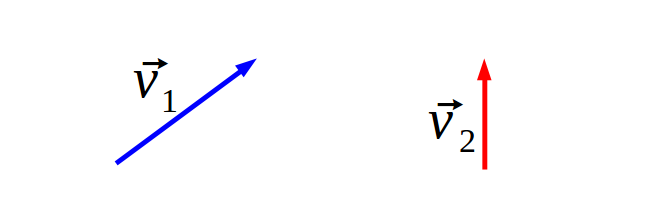
\includegraphics[width=\textwidth]{../figures/1_4-5Quiz.png}
\end{center}
\end{frame}

\begin{frame}{Quiz}
\begin{center}
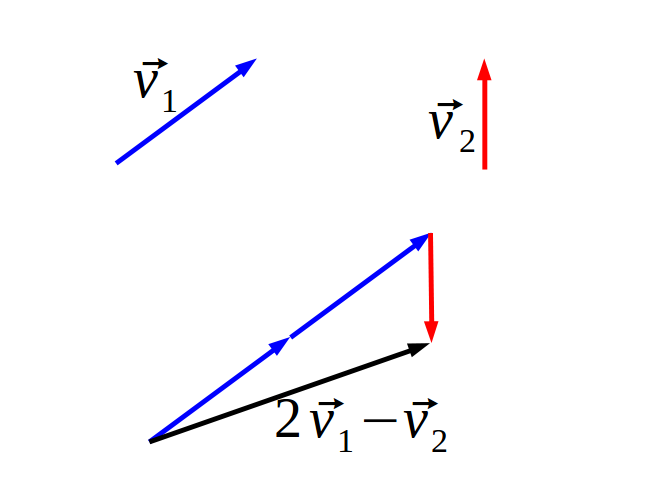
\includegraphics[width=\textwidth]{../figures/1_4-5QuizAns.png}
\end{center}
\end{frame}

\begin{frame}{Velocity}
\begin{itemize}
\item<1-> You all know the story of the tortoise and the hare right?
\item<2-> Which one ran the fastest? In other words which one had the highest speed?
\begin{itemize}
   \item<3-> The hare
\end{itemize}
\item<4-> Which one had the highest average speed?
\begin{itemize}
   \item<5-> The tortoise
\end{itemize}
\end{itemize}
\end{frame}

\begin{frame}{Velocity}
\begin{equation*}
\mathrm{average~speed} = \frac{\mathrm{distance~traveled}}{\mathrm{time~interval~spent~traveling}} = \frac{d}{\Delta t}
\end{equation*}
\begin{itemize}
\item<1-> Group question race...
\item<2-> If you drive 10 miles in 15 minutes what is your average speed in mph?
   \uncover<3>{
\begin{equation*}
   \mathrm{average~speed} = \frac{10~\rm{mi}}{1/4~\rm{hr}} = 40~\rm{mph}
\end{equation*}
   }
\end{itemize}
\end{frame}

\begin{frame}{Velocity}
\begin{itemize}
   \item<1-> What is the difference between speed and velocity?
   \uncover<2>{
   \begin{equation}
      \vec{v}_{ave} = \frac{\Delta \vec{r}}{\Delta t}
   \end{equation}}
   \item<2-> Notice that $\vec{v}_{ave}$ points in the same direction as $\vec{\Delta r}$, the direction of motion.
\end{itemize}
\end{frame}

\begin{frame}{Velocity}
\begin{center}
   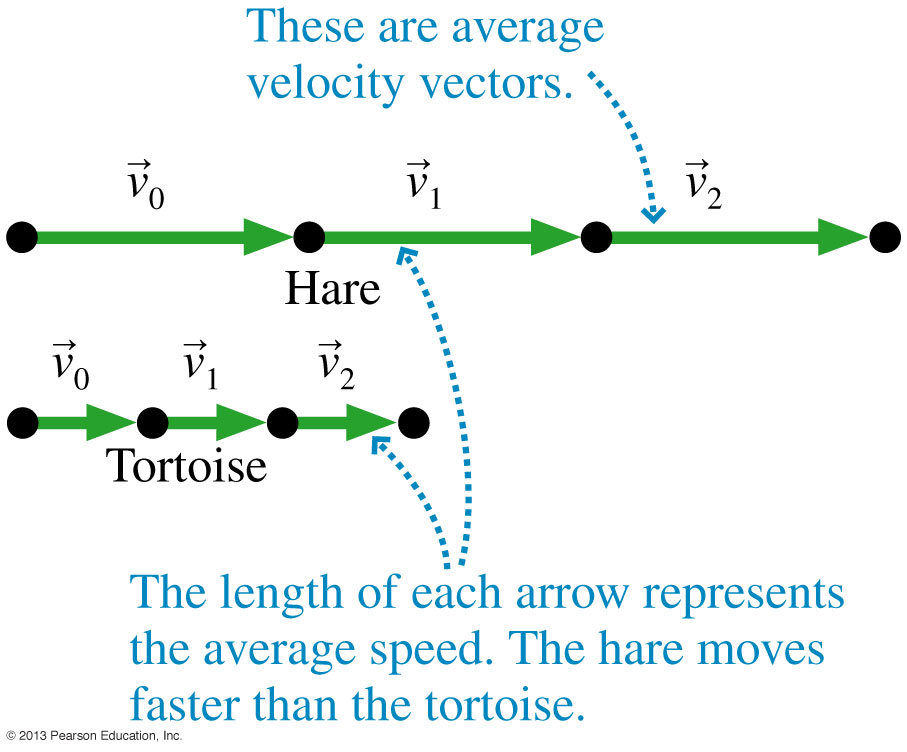
\includegraphics[width=0.5\textwidth]{../figures/01_13_Figure.jpg}
   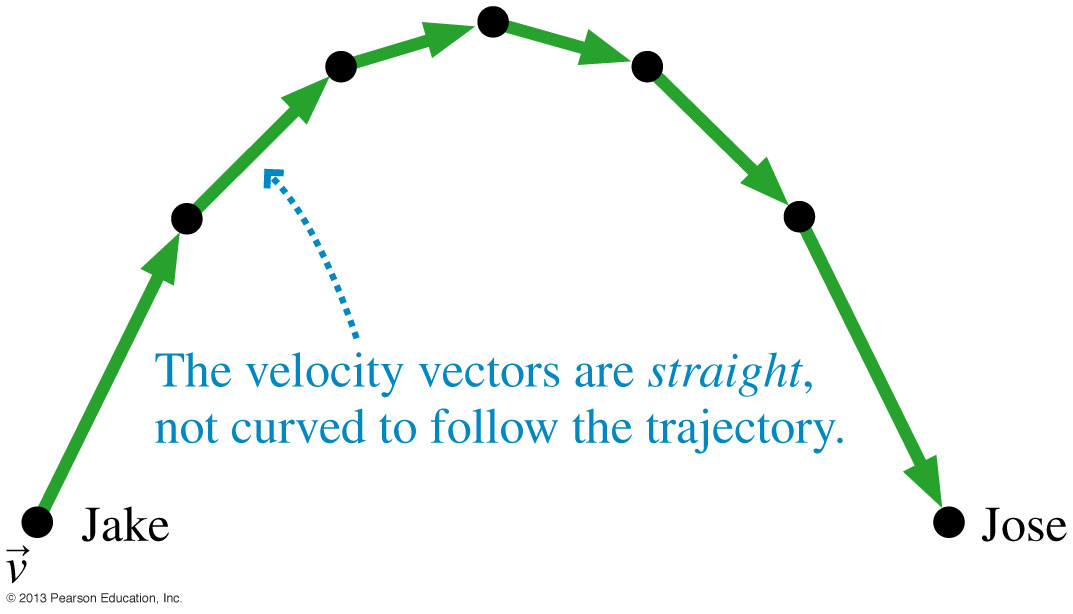
\includegraphics[width=0.5\textwidth]{../figures/01_15_Figure.jpg}
\end{center}
\end{frame}
\note{Notice that the displacement vectors can be replaces with the velocity vectors here because they are proportional. This figure also illustrates the speeding up and slowing down (in the y direction) with the arrows changing sizes.}

\begin{frame}{Quick Check}
A particle moves from position 1 to position 2 during the interval $\Delta t$. Which vector shows the particle's average velocity?
\begin{center}
   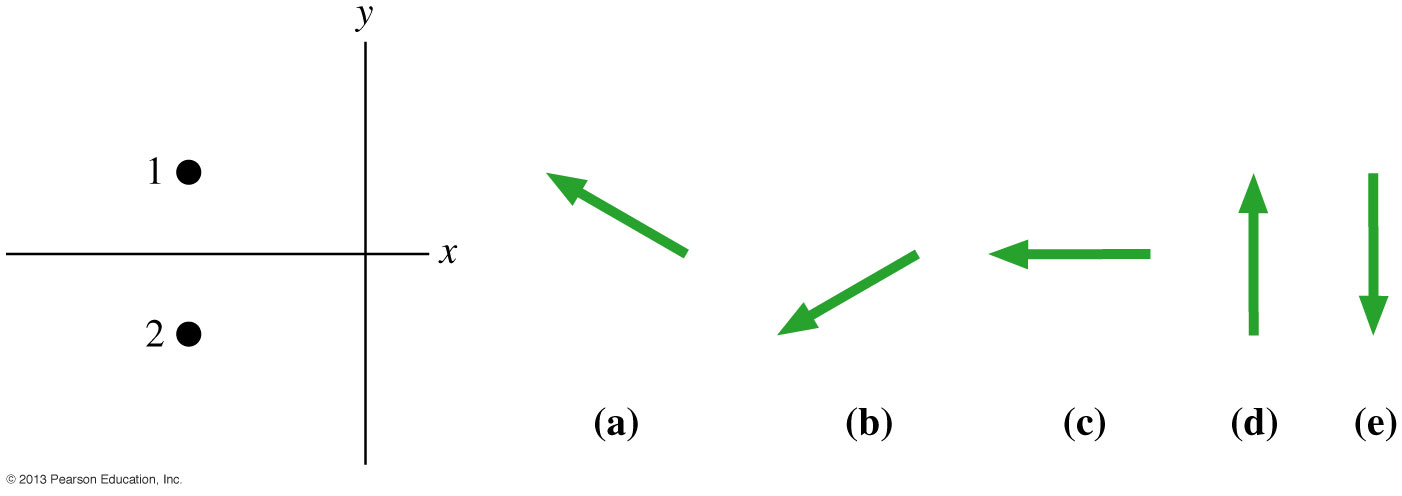
\includegraphics[width=\textwidth]{../figures/Figure_STT1_3.jpg}
\end{center}
\only<2>{\checkH{11.3cm}{6.2cm}}
\end{frame}

\begin{frame}{Quick Check}
What if it follows some specific path (draw path on the board)? Which vector shows the particle's average velocity?
\begin{center}
   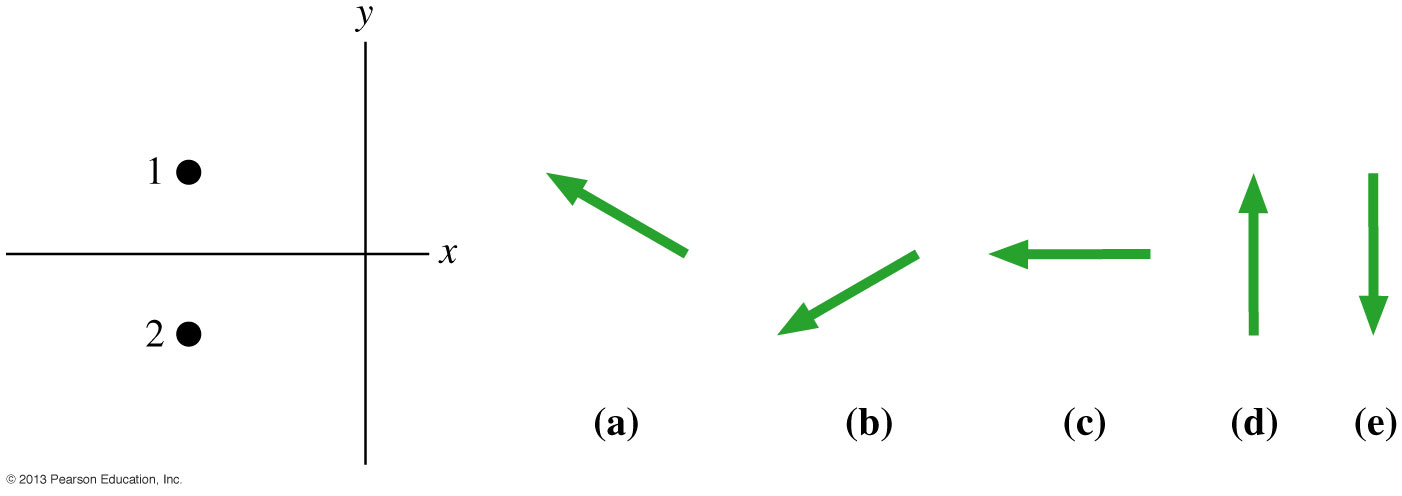
\includegraphics[width=\textwidth]{../figures/Figure_STT1_3.jpg}
\end{center}
\only<2>{\checkH{11.3cm}{6.2cm}}
\end{frame}

\begin{frame}{Linear Acceleration}
\begin{itemize}
   \item We defined velocity as the ratio $\Delta \vec{r}/\Delta t$, the rate of change of the position. To fully describe motion we also need the rate of change of velocity. We call this average acceleration.
   \begin{equation}
      \vec{a}_{ave} = \frac{\Delta \vec{v}}{\Delta t}
   \end{equation}
   \item<2-> Acceleration is a little more abstract than velocity so here's an example from every day life.
   \begin{itemize}
      \item Does anybody know how fast their vehicle can accelerate from 0 to 60 mph? My 2002 4 cylinder Ford Ranger can probably do it in about an hour... (only slightly exagerating). What then is the average acceleration of my truck in mi/hr$^2$?
      \uncover<3>{
      \begin{equation*}
         \vec{a}_{ave} = \frac{60-0~\rm{mi/hr}}{1~\rm{hr}} = 60~\rm{mi/hr^2}
      \end{equation*}}
   \end{itemize}
\end{itemize}
\end{frame}

\begin{frame}{Linear Acceleration}
\begin{columns}
\begin{column}{0.70\textwidth}
   \begin{center}
      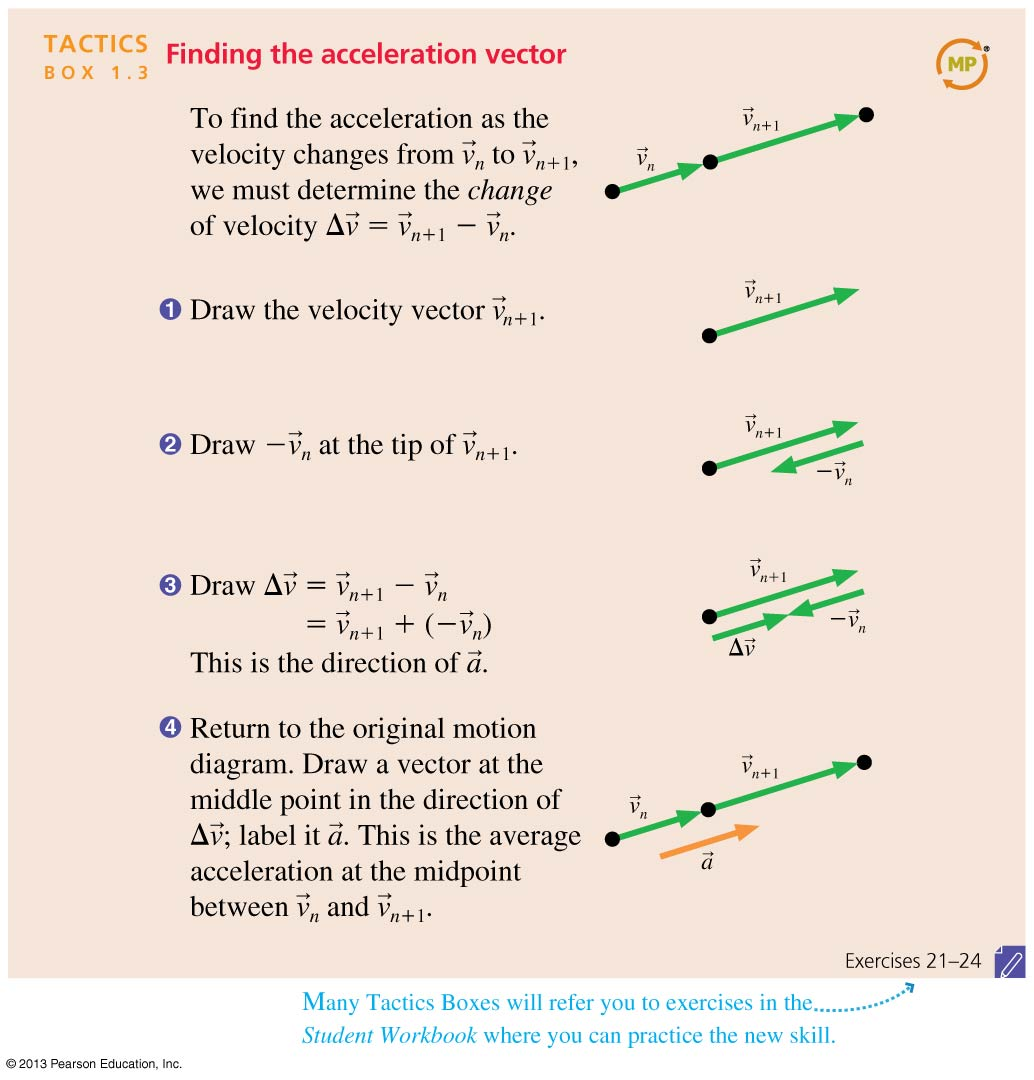
\includegraphics[height=0.9\textheight]{../figures/tactics1_3.jpg}
   \end{center}
\end{column}
\begin{column}{0.3\textwidth}
   Note that the acceleration vector goes at the dot between the vectors, not under the vector.
\end{column}
\end{columns}
\end{frame}

\begin{frame}{Linear Acceleration - Example}
\begin{columns}
\begin{column}{0.70\textwidth}
   \begin{center}
      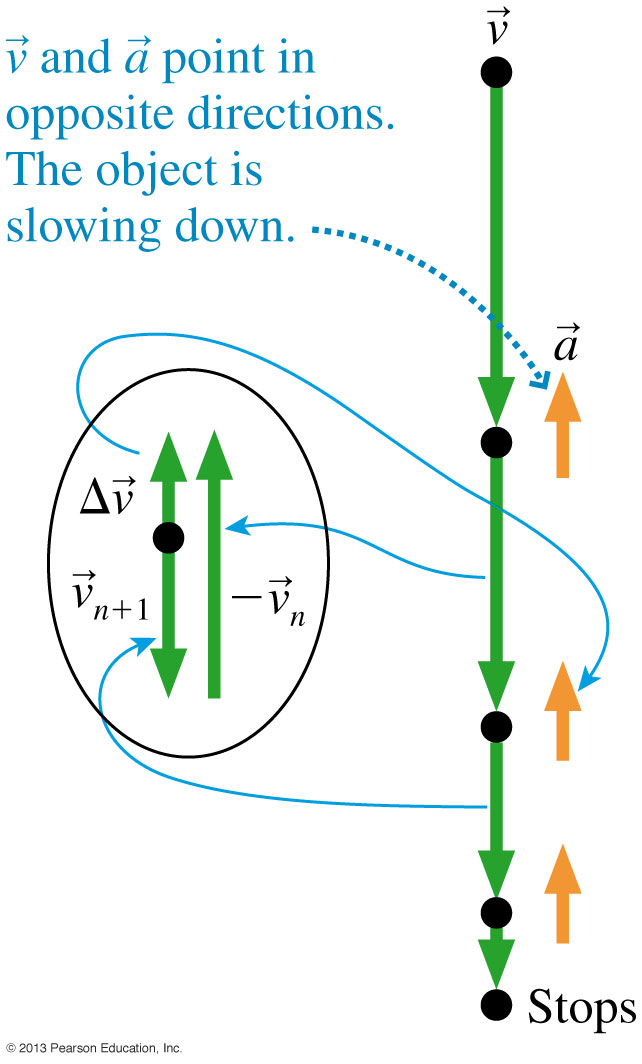
\includegraphics[height=0.9\textheight]{../figures/01_16_Figure.jpg}
   \end{center}
\end{column}
\begin{column}{0.3\textwidth}
   Motion diagram of a spaceship landing on Mars.
\end{column}
\end{columns}
\end{frame}

\begin{frame}{Quick Check}
\begin{center}
   A particle undergoes acceleration $\vec{a}$ while moving from point 1 to point 2. Which of the choices shows the velocity vector $\vec{v_2}$ as the particle moves away from point 2?
\\~\\
   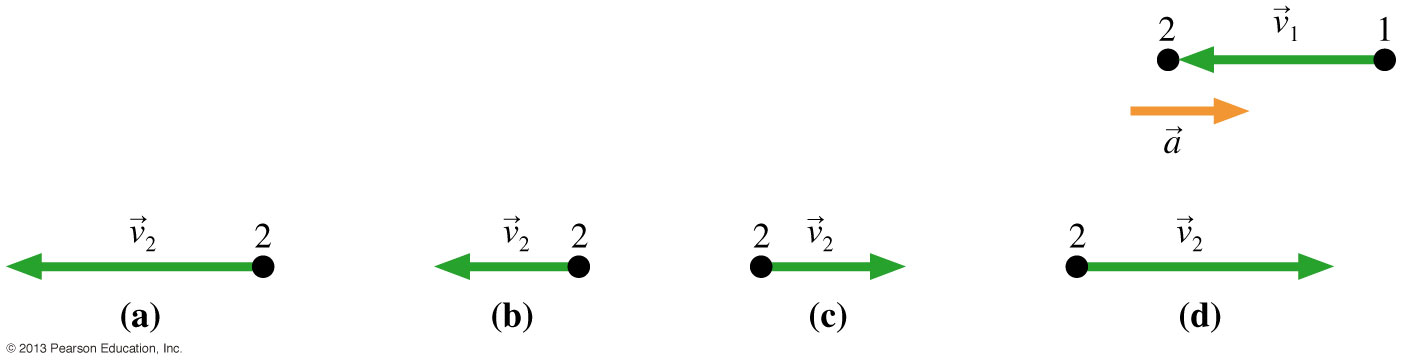
\includegraphics[width=\textwidth]{../figures/Figure_STT1_4.jpg}
   \only<2->{\checkH{4.8cm}{5.6cm}
   ~\\~\\~\\ How did you solve it?}
\end{center}
\end{frame}

\begin{frame}{Linear Acceleration - Example}
\begin{center}
   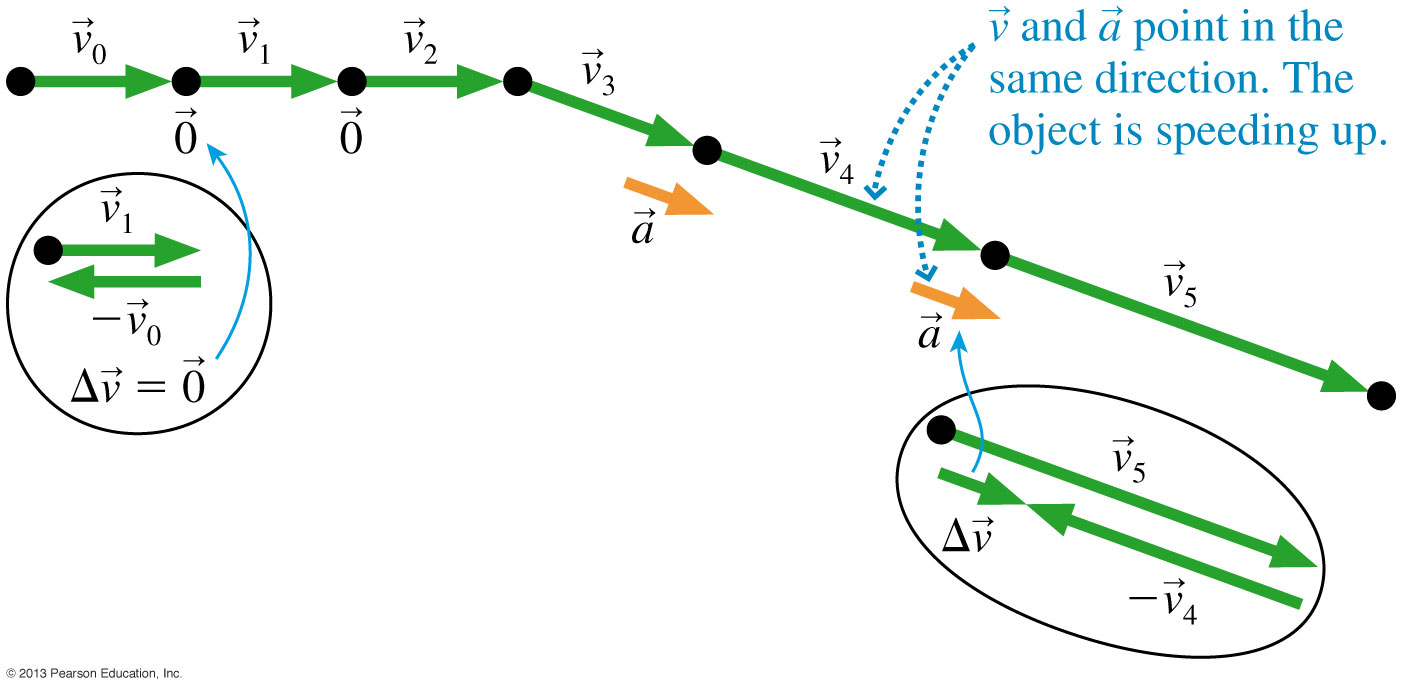
\includegraphics[width=\textwidth]{../figures/01_17_Figure.jpg}
   \\~\\ Motion diagram of skier.
\end{center}
\end{frame}

\begin{frame}{Linear Acceleration}
\begin{center}
   Build the acceleration vectors at each middle point and raise your hands when you see a pattern. \\~\\
   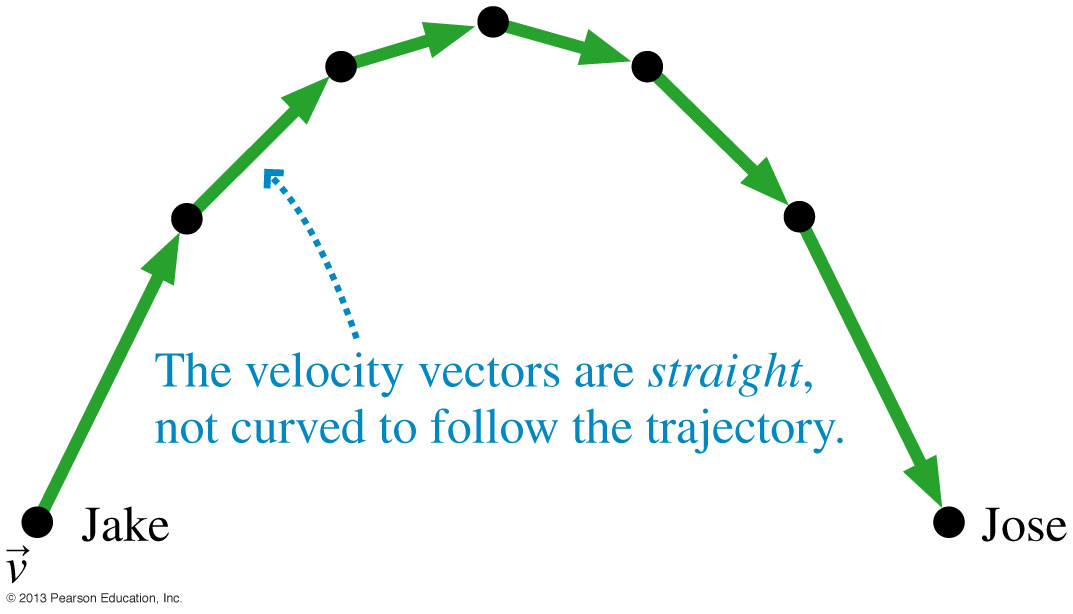
\includegraphics[width=0.7\textwidth]{../figures/01_15_Figure.jpg}
\end{center}
\end{frame}

\begin{frame}{Linear Acceleration}
\begin{itemize}
   \item Imagine throwing a ball straight into the air. On the way up what direction is the velocity/acceleration? (write your answers on the white board)
   \item<2-> What about the on way down, what is the direction of the velocity/acceleration?
   \item<3-> What about at the peak, what is the direction of the velocity/acceleration?
   \item<4-> Now draw the picture and figure it out for sure.
\end{itemize}
\end{frame}

\begin{frame}{Linear Acceleration}
\begin{columns}
\begin{column}{0.3\textwidth}
   You get the same result here, except that there was no horizontal motion to start with.
\end{column}
\begin{column}{0.70\textwidth}
   \begin{center}
      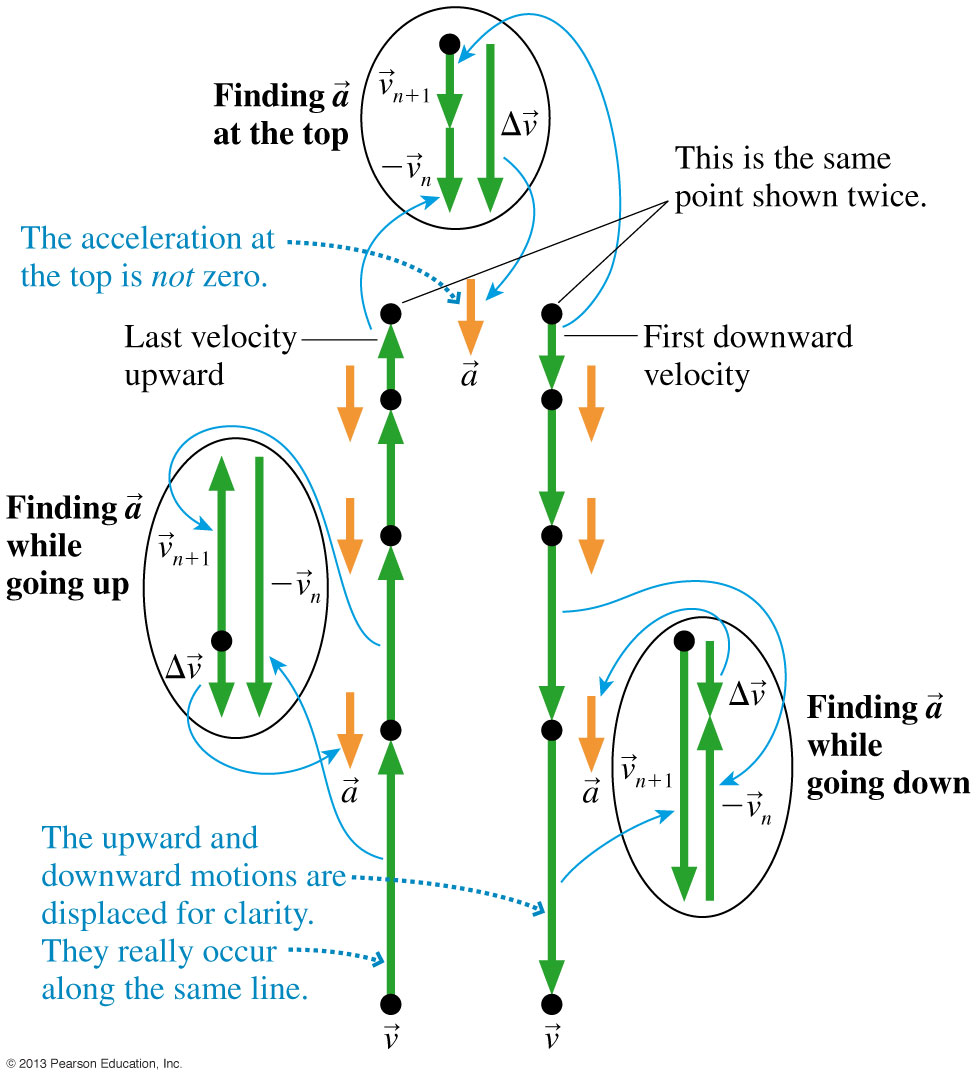
\includegraphics[height=0.9\textheight]{../figures/01_18_Figure.jpg}
   \end{center}
\end{column}
\end{columns}
\end{frame}

\begin{frame}{Reminders/Questions}
\begin{center}
   \color{blue}{\Huge Question?}
\end{center}
\begin{itemize}
   \item I have one... Have any of you had the chance to look at the Mastering Physics tutorial HW yet?
   \item Do you have any questions about that?
   \item The first HW that is due next Thursday at 11:59pm is on mastering physics.
\end{itemize}
\end{frame}

\end{document}
